% 解三棱锥顶角
% 三棱锥|立体几何|球坐标系|矢量|线面角

\pentry{高中立体几何}

\begin{figure}[ht]
\centering
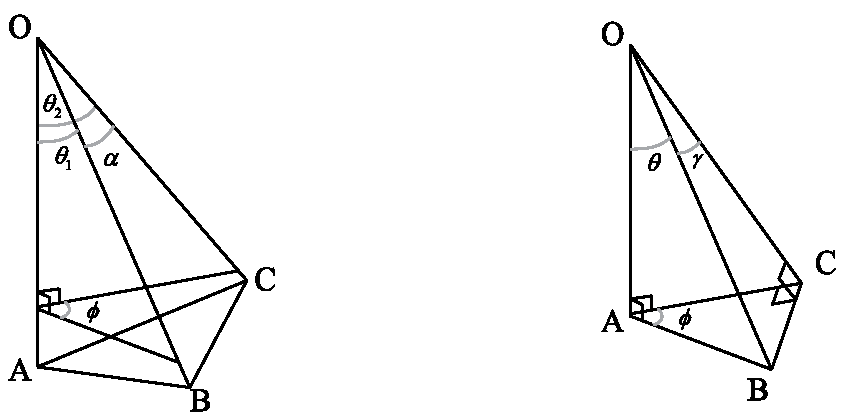
\includegraphics[width=12cm]{./figures/PrmSol_1.pdf}
\caption{(左图)已知 $\theta_1$, $\theta_2$ 和 $\phi$ 求 $\alpha$; (右图) 已知 $\theta$ 和 $\phi$ 求 $\gamma$} \label{PrmSol_fig1}
\end{figure}

我们考虑如图%链接未完成 标题: 图中的 $\theta_1$, $\theta_2$ 和 $\alpha$ 是线线角, $\phi$ 是面面角
三棱锥顶点 $O$ 处的 3 条棱和 3 个面之间的角度关系. 这里涉及了三种角: 两条棱之间的夹角(线线角) $\theta$,棱和面的夹角(线面角) $\gamma$, 以及面和面的夹角(面面角) $\phi$. 对给定的顶点, 每种角都有各有 9 个,共 9 个. 我们先不讨论底面 $ABC$ 的位置如何,如果顶点的三条棱的方向都确定, 我们就说顶点的形状确定.

显然, 我们无需知道所有 9 个角的大小才能确定顶点的形状. 这里给出一个类似于三角形余弦定理的公式, 将线线角和面面角联系起来. 线线角可以类比余弦定理中的边长, 面面角类比余弦定理中的夹角.
\begin{equation}\label{PrmSol_eq1}
\cos\alpha = \cos\theta_1 \cos\theta_2 + \sin\theta_1 \sin\theta_2 \cos\phi
\end{equation}
如果已知该式中的 4 个角中的 3 个, 就可以求出另一个角. 与余弦定理类似, 在求解 $\theta_1$ 或 $\theta_2$ 时可能存在两个解, 也可能无解. 注意如果我们交换 $\theta_1$ 和 $\theta_2$ 的值, 上式仍然满足(这相当于创造一个镜像三棱锥).

一个关于线面角的常用公式是
\begin{equation}\label{PrmSol_eq2}
\sin\gamma = \sin\phi\sin\theta_1
\end{equation}
其中 $\gamma$ 是线段 $OB$ 和三角形 $OAC$ 的线面角.

\begin{example}{已知三个线线角求线面角}
若已知 $\theta_1$, $\theta_2$ 和 $\alpha$, 则
\begin{equation}
\cos\phi = \frac{\cos\alpha - \cos\theta_1 \cos\theta_2}{\sin\theta_1 \sin\theta_2}
\end{equation}
\end{example}

\subsection{证明}
我们可以用球坐标系来证明\autoref{PrmSol_eq1}. 令极坐标 $(\theta_1, \phi_1)$ 和 $(\theta_2, \phi_2)$ 代表的两个单位矢量的坐标分别为
\begin{equation}
(\sin\theta_1\cos\phi_1, \sin\theta_1\sin\phi_1, \cos\theta_1)
\qquad
(\sin\theta_2\cos\phi_2, \sin\theta_2\sin\phi_2, \cos\theta_2)
\end{equation}
\begin{equation}
\cos\alpha = \cos\theta_1 \cos\theta_2 + \sin\theta_1 \sin\theta_2 \cos(\phi_2 - \phi_1)
\end{equation}
证毕.

再来证明\autoref{PrmSol_eq2}, 我们仍然使用球坐标, 将射线 OA 作为极轴, 面 OAC 为 $xz$ 平面, 线面角中“线” 的极坐标为 $(1, \theta, \phi)$, 该点的 $y$ 坐标为 $\sin\theta \sin\phi$ 而 $y = \sin\gamma$, 所以 $\sin\gamma = \sin\theta \sin\phi$. 证毕.